% Szablon przygotowany przez Jarosława Drapałę z dalszymi zmianami Michała Karola

% Sprawozdanie max 4 strony A4
% Repozytorium kodu powinno być dostępne przez prowadzącego
% Zalecane środowisko: Overleaf

\documentclass[10pt]{article}

\usepackage{polski}
\usepackage{graphicx}
\usepackage{hyperref}
\graphicspath{{images/}}

\usepackage{geometry}
\newgeometry{tmargin=4cm, bmargin=4cm, lmargin=3.2cm, rmargin=3.2cm} 

\usepackage{fancyhdr}
\pagestyle{fancy}

 

\begin{document}

% Szablon przygotowany przez Jarosława Drapałę z dalszymi zmianami Michała Karola

\begin{titlepage}
\begin{center}
  
  \LARGE \textsc{Politechnika Wrocławska}\\
  \vspace*{0.2cm}
  \Large \textsc{Wydział Informatyki i Telekomunikacji}\\  
  \vspace*{0.4cm}
  \centering
\includegraphics[width=0.2\textwidth]{WITlogo.png}\\
  \vspace*{0.2cm}
  \vspace*{2cm}
        
  \centerline{\rule{\textwidth}{1.2pt}}
  \vspace{0.4cm}
  \Huge\textbf{Ocena win na podstawie danych aplikacji Vivino}
  \centerline{\rule{\textwidth}{1.2pt}}
  \vspace{1cm}
  \LARGE Sprawozdanie z laboratorium\\
  \vspace{3.5cm}
  \textsc{Autor}\\
  \vspace{0.2cm}
  \textbf{Inię Nazwisko}\\
  \vspace{0.1cm}
  \Large nr albumu: \textbf{123456}\\
  \vspace{0.1cm}
  kierunek: \textbf{Informatyka}
            
            
        
        
  \vspace*{\fill}
  \Large \textit{14 styczeń 2022}
            
 \end{center}


\end{titlepage}

\begin{abstract}
Co wykonano w pracy. Skąd pobrano dane, jakie metody i modele zastosowano. Co otrzymaliśmy.
Praca przedstawia system rekomendacji win na podstawie jego cech. Dataset został pobrany z użyciem scrappera/API (!Uwaga! Nasze działania nie mogą zakłócać działania stron). Pobrane dane zostały następnie oczyszczone oraz użyto modelu/metody do predykcji oceny wina na podstawie jego cech...

\end{abstract}

\section{Wstęp -- sformułowanie problemu}
\label{sec:wstep}

Jaki jest problem?
Autor potrzebuje ocenić wino, które nie znajdują się w danych platformy Vivino. Pozwoli mu to na predykowanie oceny lokalnego wina oraz czy warto takie wino kupować czy nie...

\section{Opis danych}
Wielkość danych, opis słowny kolumn, powiązania pomiędzy cechami, zares wartości, typ zmiennej (string, categorical, int, float, etc...).

Wielkość datasetu 10000 wierszy.
Kolumna "kolor" - zmienna kategoryczna, okreśła ona kolor wina. Zbiór wartości: czerowne, białe, różowe, zielone.
...


\section{Opis rozwiązania}

Dane kto kogo zostaną pobrane ze strony \url{www.vivino.com}. Dostęp do danych uzyskano za pomocą API. Baza została zapisana w postaci ramki danych biblioteki \texttt{Pandas}. Zawiera ona informacje o 10000 winach wraz z 12 cechami je określającymi.

Używając metody \textit{XYZ} na danych uzyskano model pozwajacy na określenie oceny wina na podstawie jego koloru, rocznika, ceny oraz szczepu...

\section{Rezultaty obliczeń}

\subsection{Plan badań}
Zbiór danych zostanie podzielony na dwie części: treningową i testową w stosunku 80:20. 


\subsection{Wyniki obliczeń} 
Model oceny wina można przedstawić następującym wzorem:
\begin{equation}
\det Score = alpha * rocznik + beta * catToOneHot(kolor) + gamma * catToOneHot(szczep) 
\label{eq:wzor_wazny}
\end{equation}
gdzie $catToDec$ to funkcja mapująca dane kategoryczne na reprezentację one-hot.

Na rys. \ref{fig:korelacje} pokazany jest przykładowy wykres. 
\begin{figure}[!hbt]
\begin{center}
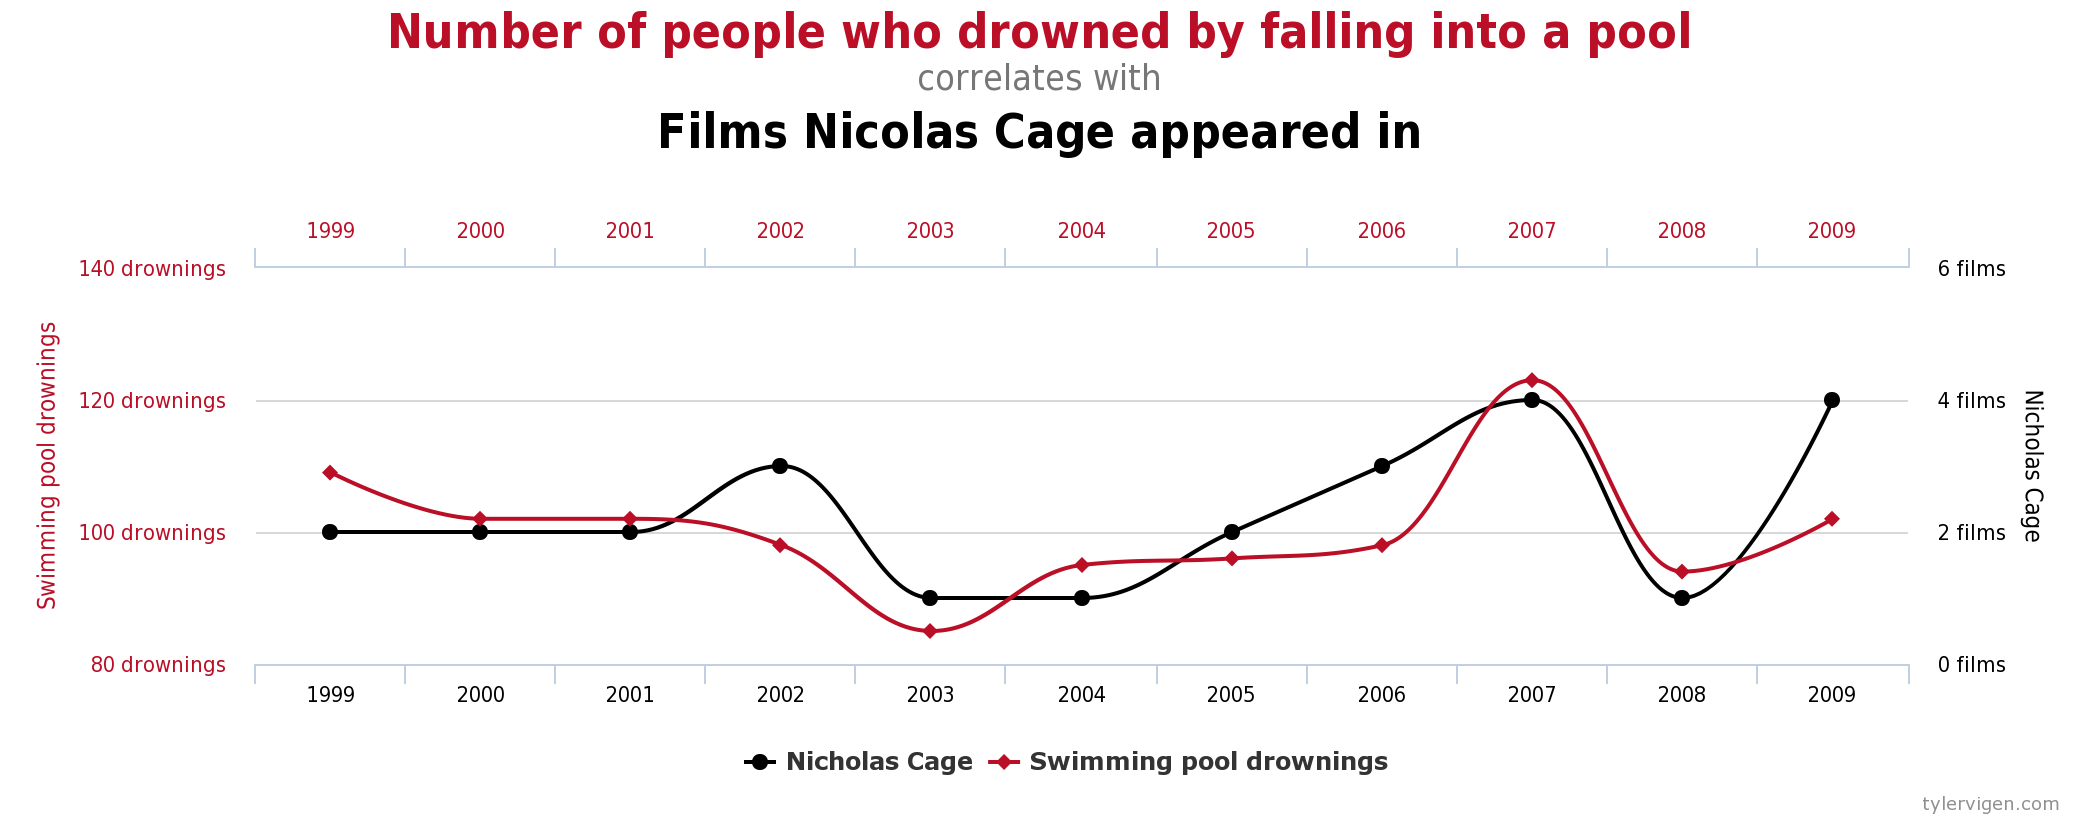
\includegraphics[width=0.8\linewidth]{rys1.png}
\caption{Fałszywe korelacje}
\label{fig:korelacje}
\end{center}
\end{figure}

Oznacza to że szczep wina jest nieistotny, natomiast najważniejszym elementem w ocenie wina jest cena.

Podsumowując, symulacje ujawniają że wg. (\ref{eq:wzor_wazny}) ocena wina na półce powinna byc bardzo prosta...
Jakie metryki użyto do oceny modelu/metody...

\section{Wnioski}
Przedstawiona metoda pozwala na przygotowanie modelu i ten model jest wytrzymały na nowe dane. Uzyskane model daje szczególnie ciekawe dane w asortymencie win do 20 zł do 30 zł w Biedronce, pokazując że wina w tym zakresie cenowym osiągają szczególnie wysokie oceny...

\appendix
\section{Dodatek}
Kody źródłowe(utrzymane w konwencji języka Python wraz z instrukcjmi uruchomienia) umieszczone zostały w repozytorium github:

\noindent \url{https://github.com/jdrapala/sieci_zlozone}.


\end{document}